%-----------------------------------------------------------------------------%
\chapter{\babDua}
%-----------------------------------------------------------------------------%

%-----------------------------------------------------------------------------%
\section{Perangkat Lunak (\f{Software})}
%-----------------------------------------------------------------------------%
Perangkat lunak adalah serangkaian instruksi, data, atau program yang digunakan untuk mengoperasikan komputer dan menjalankan tugas-tugas tertentu \cite{gee23}. Perangkat lunak memberikan instruksi kepada perangkat keras (hardware) tentang apa yang harus dilakukan, bertindak sebagai perantara antara pengguna dan perangkat keras. Tanpa perangkat lunak, sebagian besar hardware komputer tidak akan berfungsi. Sebagai contoh, prosesor membutuhkan instruksi dari perangkat lunak untuk melakukan perhitungan, dan monitor membutuhkan driver perangkat lunak untuk menampilkan gambar. Perangkat lunak tidak memiliki wujud fisik dan bersifat intangible, berbeda dengan hardware yang dapat disentuh. Perangkat lunak didistribusikan dalam berbagai bentuk, seperti program yang diinstal pada komputer, aplikasi mobile, aplikasi web, dan embedded systems.

\subsection{Perangkat Lunak Sistem}
Perangkat lunak sistem merupakan fondasi yang memungkinkan perangkat lunak aplikasi dan pengguna berinteraksi dengan perangkat keras \cite{gee23}. Fungsinya antara lain mengelola sumber daya sistem seperti memori, prosesor, dan perangkat input/output. Perangkat lunak sistem juga menyediakan layanan dasar seperti sistem file, manajemen proses, dan antarmuka pengguna. Contoh perangkat lunak sistem meliputi:

\begin{enumerate}
	\item \bo{Sistem Operasi (\f{Operating System}):} Bertindak sebagai platform untuk menjalankan perangkat lunak aplikasi. Sistem operasi mengelola sumber daya hardware, menyediakan antarmuka pengguna, dan menjalankan layanan sistem. Contoh: Microsoft Windows, macOS, Linux, Android, iOS.

	\item \bo{Driver Perangkat Keras (\f{Device Drivers}):} Program yang memungkinkan sistem operasi untuk berkomunikasi dengan perangkat keras tertentu, seperti printer, kartu grafis, kartu suara, webcam, dan mouse. Setiap perangkat keras membutuhkan driver khusus agar dapat berfungsi dengan baik.

\end{enumerate}

\begin{figure}[!htb]
	\begin{minipage}{0.52\textwidth}
		\centering
		
\includegraphics[width=0.8\linewidth]
		{assets/pics/windows.png}
	\end{minipage}\hfill
	\begin{minipage}{0.38\textwidth}
		
\includegraphics[width=0.4\linewidth]
		{assets/pics/linux.png}
	\end{minipage}
	\caption{Sistem Operasi Windows \& Linux}
\end{figure}

\subsection{Perangkat Lunak Aplikasi}
Perangkat lunak aplikasi dirancang untuk memenuhi kebutuhan spesifik pengguna \cite{gee23}. Kategori perangkat lunak aplikasi sangat luas dan beragam, berfokus pada penyelesaian tugas-tugas tertentu untuk pengguna. Perangkat lunak aplikasi berjalan di atas sistem operasi dan memanfaatkan layanan yang disediakan oleh sistem operasi.

\begin{itemize}

	\item \bo{Pengolah Kata (\f{Word Processors}):} Digunakan untuk membuat dan mengedit dokumen teks, memformat teks, menambahkan gambar dan tabel, dan melakukan tugas-tugas pengolah kata lainnya. Contoh: Microsoft Word, Google Docs
	\item \bo{Perangkat Lunak Desain Grafis:} Digunakan untuk membuat dan mengedit gambar, ilustrasi, dan desain visual lainnya. Contoh: Adobe Photoshop, GIMP, Inkscape.

\end{itemize}

\begin{figure}[!htb]
	\begin{minipage}{0.5\textwidth}
		\centering
		
\includegraphics[width=0.3\linewidth]
		{assets/pics/word.png}
	\end{minipage}
	\begin{minipage}{0.5\textwidth}
		
\includegraphics[width=0.3\linewidth]
		{assets/pics/photoshop.png}
	\end{minipage}
	\caption{Perangkat lunak aplikasi}
\end{figure}

\subsection{Proses Kompilasi dan Eksekusi Perangkat Lunak}
Proses menjalankan perangkat lunak melibatkan dua tahap utama: kompilasi dan eksekusi. Kedua tahap ini penting untuk mengubah kode sumber yang dapat dibaca manusia menjadi instruksi yang dapat dieksekusi oleh mesin. Berikut penjelasan lebih detail, dibagi menjadi dua sub-bagian:

\subsubsection{Proses Kompilasi}
Proses kompilasi mengubah kode sumber (source code) yang ditulis dalam bahasa pemrograman tingkat tinggi menjadi kode mesin (machine code) atau kode objek (object code) \cite{tut24}. Proses ini melibatkan beberapa tahapan, yang masing-masing dilakukan oleh program utilitas yang berbeda:

\begin{enumerate}
	\item \bo{Preprocessing:} Tahap pertama dalam proses kompilasi adalah preprocessing. Preprocessor menangani direktif-direktif preprocessor yang dimulai dengan simbol \#, seperti \#include dan \#define dalam kode sumber.
	\item \bo{Compilation:} Pada tahap ini, compiler menerjemahkan kode sumber yang telah diproses menjadi assembly code. Assembly code adalah representasi mnemonic dari kode mesin, yang lebih mudah dibaca oleh manusia. Kompiler melakukan analisis sintaks dan semantik untuk memastikan kode sumber valid dan sesuai dengan aturan bahasa pemrograman. Kompiler juga melakukan optimasi kode untuk meningkatkan kinerja program.
	\item \bo{Assembly:} Assembler menerjemahkan assembly code menjadi kode objek (object code). Kode objek adalah representasi biner dari instruksi mesin, tetapi belum siap untuk dieksekusi. Kode objek berisi instruksi mesin dan data, tetapi belum terhubung dengan library eksternal.
	\item \bo{Linking:} Linker menggabungkan kode objek dari berbagai file sumber dan library menjadi satu file executable. Linker menyelesaikan referensi eksternal, mengalokasikan alamat memori untuk variabel dan fungsi, dan menghubungkan kode objek dengan library yang dibutuhkan. Output dari tahap linking adalah file executable yang siap dieksekusi.
\end{enumerate}

\begin{figure}
	\centering
	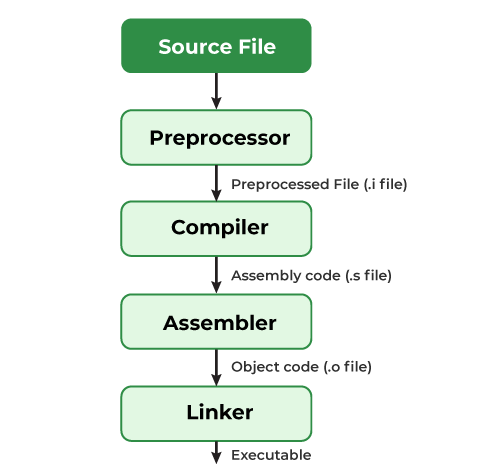
\includegraphics[width=0.35\textheight]
	{assets/pics/program_compile.png}
	\caption{Alur kompilasi program \cite{tut24}}
\end{figure}

\subsubsection{Proses Eksekusi}
Setelah program dikompilasi menjadi file executable, proses eksekusi dimulai \cite{Dan24}. Proses eksekusi melibatkan beberapa tahapan yang dilakukan oleh sistem operasi:
\begin{enumerate}
	\item \bo{Loading:} Loader yaitu sebuah komponen dari sistem operasi, memuat file executable ke dalam memori utama (RAM). Loader mengalokasikan ruang memori yang dibutuhkan oleh program, memuat instruksi dan data ke dalam memori, dan menginisialisasi program untuk eksekusi.
	\item \bo{Eksekusi:} Setelah program dimuat ke dalam memori, prosesor mulai mengeksekusi instruksi-instruksi yang terdapat dalam program. Prosesor mengambil instruksi satu per satu dari memori, mendekode instruksi, dan mengeksekusinya. Siklus ini berulang hingga program selesai dijalankan atau dihentikan.
	\item \bo{Terminasi:} Program berakhir ketika mencapai instruksi terminasi atau ketika terjadi kesalahan yang menyebabkan program berhenti secara paksa. Sistem operasi kemudian membebaskan sumber daya yang digunakan oleh program, seperti memori dan file.
\end{enumerate}

\begin{figure}
	\centering
	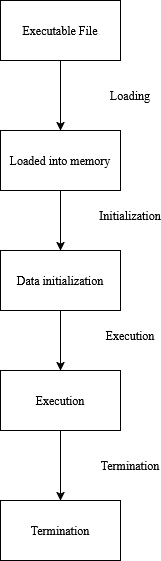
\includegraphics[height=0.4\textheight]
	{assets/pics/program_execution.png}
	\caption{Alur eksekusi program \cite{Dan24}}
\end{figure}


\section{\f{Software Control Flow}}
Alur kendali perangkat lunak (software control flow) merupakan aspek fundamental dalam eksekusi program, merepresentasikan urutan instruksi yang dieksekusi oleh prosesor untuk mencapai tujuan fungsionalitas program \cite{cod23}. Memahami software control flow adalah krusial dalam analisis kode, terutama dalam reverse engineering karena memungkinkan pemetaan jalur eksekusi, identifikasi bottleneck, dan potensi kerentanan. Dalam konteks ini, control flow bukan hanya sekadar urutan instruksi, tetapi juga representasi logis dari bagaimana program merespons input, kondisi, dan interaksi dengan sistem operasi. Pemahaman yang komprehensif terhadap aspek ini memberikan dasar yang kuat dalam menganalisis perilaku program, baik secara statis melalui analisis kode sumber dan intermediate representation, maupun secara dinamis melalui observasi eksekusi runtime.

\subsection{\f{Control Flow Instructions}}
Instruksi alur kendali (control flow instructions) adalah mekanisme fundamental yang menentukan urutan eksekusi instruksi dalam suatu program \cite{cod23}. Instruksi ini memungkinkan program untuk membuat keputusan, mengulang blok kode, dan melompat ke bagian kode yang berbeda. Cara instruksi-instruksi ini direpresentasikan dan diimplementasikan sangat bergantung pada tingkat bahasa pemrograman yang digunakan. Secara umum, kita membedakan antara bahasa tingkat tinggi dan bahasa tingkat rendah.

\subsubsection{\f{High Level Languages}}
Bahasa pemrograman tingkat tinggi (high-level languages), seperti Python, Java, C++, dan JavaScript, menyediakan abstraksi yang jauh dari detail hardware. Bahasa-bahasa ini fokus pada kemudahan penulisan dan pemahaman kode oleh programmer, dengan menggunakan sintaks yang lebih dekat dengan bahasa manusia. Instruksi control flow dalam bahasa tingkat tinggi diimplementasikan melalui konstruksi yang intuitif, seperti \textit{if, else, for}, dan \textit{while}.

\paragraph{Conditional Instructions:}
\begin{itemize}
	\item \bi{if statement:} Memungkinkan program membuat keputusan berdasarkan kondisi.
	      \begin{minted}
{c}     
if (x > 10) {
 std::cout << "x lebih besar dari 10" << std::endl;
}
    \end{minted}

	\item \bi{if-else statement:} Menyediakan jalur alternatif jika kondisi \textit{if} tidak terpenuhi.
	      \begin{minted}
{c}     
if (score >= 70) {
 std::cout << "Lulus" << std::endl;
} else {
 std::cout << "Tidak Lulus" << std::endl;
}
    \end{minted}
	\item \bi{switch statement:} Memungkinkan percabangan ke banyak kasus.
	      \begin{minted}
{c}     
int day = 2;
switch (day) {
 case 1:
 std::cout << "Senin" << std::endl;
 break;
 case 2:
 std::cout << "Selasa" << std::endl;
 break;
 default:
 std::cout << "Hari lain" << std::endl;
}
    \end{minted}
\end{itemize}

\paragraph{Loop Instructions:}
\begin{itemize}
	\item \bi{for loop:} Mengeksekusi blok kode sejumlah kali tertentu.
	      \begin{minted}
{c}     
for (int i = 0; i < 5; i++) {
 std::cout << i << std::endl;
}
    \end{minted}
	\item \bi{while loop:} Mengeksekusi blok kode selama kondisi tertentu terpenuhi.
	      \begin{minted}
{c}     
int count = 0;
while (count < 5) {
 std::cout << count << std::endl;
 count++;
}
    \end{minted}
\end{itemize}

\paragraph{Jump Instructions (Indirect - Function Calls):}
\begin{itemize}
	\item \bi{Function call:} Memindahkan kontrol ke fungsi lain dan kembali setelah selesai.
	      \begin{minted} {c}
void myFunction() {
 std::cout << "Hello" << std::endl;
}
int main() {
 myFunction();
 return 0;
}
    \end{minted}
\end{itemize}

\subsubsection{\f{Low Level Languages}}
Bahasa pemrograman tingkat rendah (low-level languages), seperti Assembly language, bekerja lebih dekat dengan hardware. Instruksi-instruksinya langsung dikodekan ke dalam instruksi mesin yang dapat dieksekusi oleh prosesor. Bahasa tingkat rendah memberikan kontrol yang lebih besar atas hardware, tetapi seringkali lebih kompleks dan sulit untuk dipahami oleh manusia. Instruksi control flow pada tingkat ini melibatkan kode operasi (opcode) yang merepresentasikan operasi jump dan perbandingan secara langsung \cite{USC24}. Dalam bagian ini, contoh akan difokuskan pada bahasa x86 Assembly.

\paragraph{Conditional Instructions:}
\begin{itemize}
	\item \bi{cmp (compare):} Membandingkan dua nilai dan mengatur flags (bendera) kondisi.
	      \begin{minted}
{asm}     
cmp eax, 10
    \end{minted}
	\item \bi{jle, jge, je, jne (conditional jumps):} Melompat ke label lain jika flags kondisi memenuhi syarat.
	      \begin{minted}
{asm}     
jle less_or_equal ; Lompat jika kurang dari atau sama dengan
jne not_equal ; Lompat jika tidak sama dengan
    \end{minted}
\end{itemize}

\paragraph{Loop Instructions (Implementasi dengan Conditional Jumps):}
\begin{itemize}
	\item Menggunakan kombinasi instruksi perbandingan, pengurangan counter, dan conditional jump untuk membuat loop.
	      \begin{minted}
{asm}     
mov ecx, 5 ; set counter loop
loop_start:
; instruksi dalam loop
cmp ecx, 0
jne loop_start
    \end{minted}
\end{itemize}

\paragraph{Jump Instructions (Direct):}
\begin{itemize}
	\item \bi{jmp (unconditional jump):} Lompat ke label tanpa syarat.
	      \begin{minted}
{asm}     
jmp target_label
    \end{minted}
\end{itemize}

\paragraph{Jump Instructions (Indirect - function calls):}
\begin{itemize}
	\item \bi{call:} Melompat ke alamat fungsi dan menyimpan alamat return.
	      \begin{minted}
{asm}     
call function_address
    \end{minted}
	\item \bi{ret:} Mengembalikan kontrol dari fungsi.
	      \begin{minted}
{asm}     
ret
    \end{minted}
\end{itemize}

\subsection{Control Flow Graph}
Graf Alur Kendali (Control Flow Graph atau CFG) adalah representasi grafis dari alur kendali suatu program. CFG memvisualisasikan bagaimana eksekusi program berjalan melalui berbagai blok kode, menggambarkan urutan eksekusi, percabangan, dan perulangan \cite{Myi19}. CFG sangat penting dalam analisis statis kode, reverse engineering, dan optimisasi kode \cite{Rou05}. Dalam CFG, blok dasar (basic blocks) direpresentasikan sebagai simpul (nodes) dan transisi antar blok dasar direpresentasikan sebagai sisi/garis (edges). Contohnya dapat dilihat pada Gambar \ref{F:graph}.

\begin{figure}
	\centering
	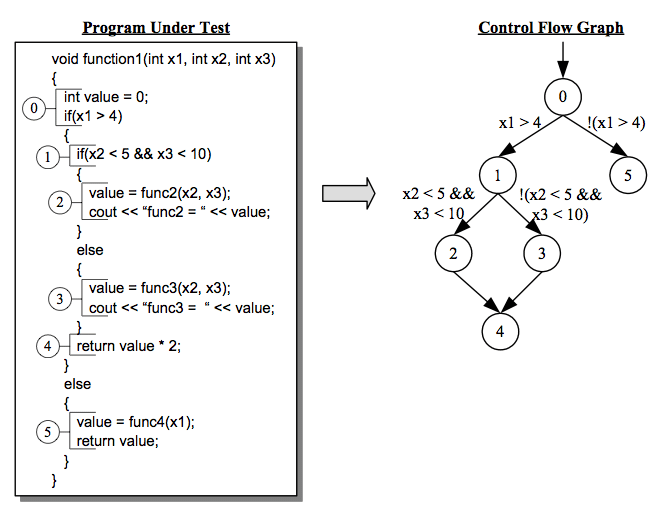
\includegraphics[width=1\textwidth]
	{assets/pics/control_flow_graph.png}
	\caption{Contoh Control Flow Graph \cite{Gom}}
	\label{F:graph}
\end{figure}

%-----------------------------------------------------------------------------%
\section{Rekayasa balik (\f{Reverse Engineering})}
%-----------------------------------------------------------------------------%
Rekayasa balik (reverse engineering) adalah proses menganalisis suatu sistem, baik perangkat lunak, perangkat keras, atau sistem lainnya, untuk mengidentifikasi komponen-komponennya dan interaksi antar komponen, serta memahami cara kerja sistem tersebut tanpa akses ke dokumentasi asli atau kode sumber \cite{Has18}.  Tujuannya beragam, mulai dari pemahaman fungsionalitas, analisis keamanan untuk menemukan kerentanan, pemulihan desain, hingga modifikasi dan peningkatan sistem. Rekayasa balik dapat diterapkan pada berbagai skenario, misalnya untuk menganalisis malware, memahami format file yang tidak terdokumentasi, mempelajari teknik yang digunakan oleh pesaing atau modifikasi fungsionalitas perangkat lunak.

\subsection{Jenis Analisis Rekayasa Balik}
\begin{enumerate}
	\item \bo{Analisis Statis}\\
	      Analisis statis melibatkan pemeriksaan kode tanpa menjalankannya. Analisis statis berfokus pada struktur dan logika kode, mencari pola dan kerentanan \cite{Sec19}. Alat yang digunakan dalam analisis statis meliputi:
	      \begin{itemize}
		      \item \bi{Disassembler:}  Menerjemahkan kode mesin menjadi assembly code, sebuah representasi kode yang lebih mudah dibaca oleh manusia. Contoh: IDA Pro, Ghidra, Radare2.
		      \item \bi{Decompiler:}  Menerjemahkan kode mesin atau bytecode kembali ke kode sumber tingkat tinggi (misalnya, C++ atau Java). Decompiler membantu memahami logika program secara lebih mudah.
		      \item \bi{Code Analysis Tools:}  Alat yang digunakan untuk menganalisis kode secara otomatis, mencari kerentanan keamanan, pola kode yang buruk, dan masalah lainnya.
	      \end{itemize}

	      \begin{figure}
		      \centering
		      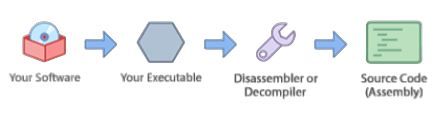
\includegraphics[width=.75\textwidth]
		      {assets/pics/program_decompile.png}
		      \caption{Dekompilasi Aplikasi \cite{Ore06}}
	      \end{figure}
	\item \bo{Analisis Dinamik} \\
	      Analisis dinamis melibatkan menjalankan program dan mengamati perilakunya. Analisis dinamis berfokus pada bagaimana program berinteraksi dengan lingkungannya, mencari kerentanan runtime dan memahami alur eksekusi \cite{Sec19}.  Alat yang digunakan dalam analisis dinamis meliputi:
	      \begin{itemize}
		      \item \bi{Debugger:} Memungkinkan eksekusi program secara terkontrol, memeriksa nilai variabel, dan melacak alur eksekusi. Contoh: x64dbg, OllyDbg, GDB.
		      \item \bi{Profiler:} Mengukur penggunaan sumber daya program, seperti waktu eksekusi, penggunaan memori, dan akses file. Profiler membantu mengidentifikasi bottleneck kinerja.
	      \end{itemize}
\end{enumerate}

\subsection{\f{Tampering}}
\f{Tampering} merupakan suatu proses mengubah kode aplikasi untuk mempengaruhi perilakunya. Contoh Tampering perangkat lunak adalah mengubah kode aplikasi agar dapat melewati proses autentikasi dalam perangkat lunak tersebut. Hal ini dapat dilakukan dengan memodifikasi control flow pada proses autentikasi dalam programnya. \\
\f{Tampering} bisa dilakukan pada berbagai tingkatan dan bagian dari perangkat lunak, termasuk
\begin{itemize}
	\item \bo{Kode biner (\textit{executable code}):} Mengubah instruksi mesin yang dijalankan oleh prosesor. Hal ini bisa digunakan untuk mematikan fitur tertentu, menambahkan fitur baru, mengubah perilaku program, atau menyisipkan kode berbahaya.
	\item \bo{Data} Mengubah data konfigurasi, aset game, atau data sensitif lainnya yang digunakan oleh program.
	\item \bo{Pustaka (\textit{Library}):} Memodifikasi library yang digunakan oleh program untuk mengubah fungsionalitasnya.
	\item \bo{Sumber Daya (\textit{Resources}):} Mengubah teks, gambar, atau elemen lain yang digunakan oleh program.
\end{itemize}


\subsection{Alat-alat untuk Rekayasa Balik}
\begin{itemize}
	\item \bo{IDA Pro (Interactive Disassembler Pro):} Disassembler dan debugger komersial yang sangat populer dan powerful. IDA Pro mendukung berbagai arsitektur prosesor dan sistem operasi, menyediakan antarmuka yang canggih untuk analisis kode, dan mendukung plugin untuk ekstensibilitas \cite{Hex91}.
	      \begin{figure}
		      \centering
		      
\includegraphics[width=.6\textwidth]
		      {assets/pics/IDA_pro.png}
		      \caption{IDA Pro \cite{Hex91}}
	      \end{figure}
	\item \bo{Ghidra:} Framework reverse engineering open-source yang dikembangkan oleh NSA (National Security Agency). Ghidra menawarkan fitur yang setara dengan IDA Pro, termasuk disassembler, decompiler, dan debugger. Ghidra juga mendukung scripting dan ekstensibilitas melalui plugin \cite{Nat19}.
	      \begin{figure}
		      \centering
		      
\includegraphics[width=.4\textwidth]
		      {assets/pics/Ghidra.png}
		      \caption{Ghidra \cite{Nat19}}
	      \end{figure}
	\item \bo{x64dbg:} Debugger open-source untuk platform Windows. x64dbg menyediakan antarmuka yang modern dan user-friendly, serta mendukung plugin dan scripting. x64dbg fokus pada analisis malware dan reverse engineering aplikasi Windows \cite{Dun14}.
	      \begin{figure}
		      \centering
		      
\includegraphics[width=.5\textwidth]
		      {assets/pics/x64Dbg.png}
		      \caption{x64dbg \cite{Dun14}}
	      \end{figure}
\end{itemize}

%-----------------------------------------------------------------------------%
\section{\f{Obfuscation}}
%-----------------------------------------------------------------------------%
Obfuscation adalah teknik yang digunakan untuk mengubah kode sumber atau kode mesin menjadi bentuk yang lebih sulit dipahami oleh manusia, tanpa mengubah fungsionalitas program. Tujuan utama obfuscation adalah untuk mempersulit analisis dan reverse engineering, melindungi kekayaan intelektual, dan meningkatkan keamanan aplikasi. Obfuscation tidak membuat kode menjadi tidak mungkin untuk di-reverse engineer, tetapi meningkatkan waktu dan usaha yang dibutuhkan untuk melakukannya, sehingga membuat reverse engineering menjadi kurang menarik bagi penyerang \cite{Jin24}.

\subsection{Manfaat \f{Obfuscation}}
\begin{itemize}
	\item \bo{Meningkatkan Keamanan:} Obfuscation mempersulit penyerang untuk memahami logika program, menemukan kerentanan, dan memodifikasi kode untuk tujuan jahat. Obfuscation dapat melindungi algoritma penting, kunci enkripsi, dan data sensitif lainnya.
	\item \bo{Melindungi Kekayaan Intelektual:} Obfuscation dapat mempersulit pesaing untuk mencuri kode sumber, meniru fungsionalitas program, dan melanggar hak cipta. Ini penting terutama untuk perangkat lunak komersial dan aplikasi yang mengandung algoritma atau teknologi yang unik.
\end{itemize}

\subsection{Jenis-jenis \f{Obfuscation}}
Obfuscation dapat dilakukan pada diterapkan pada kode sumber, bytecode, atau kode biner.
\subsubsection{Kode Sumber \f{Obfuscation}}
Teknik ini mengubah kode sumber yang dapat dibaca manusia, sehingga sulit dipahami tanpa memengaruhi fungsinya \cite{Jin24}.
\begin{itemize}
	\item \bi{Layout obfuscation:} mengubah tampilan kode.
	      \begin{itemize}
		      \item \bi{Scrabling identifiers \cite{Cha04}:} mengubah nama fungsi dan variabel.
		      \item \bi{Changing formatting \cite{Bal11}:} menambahkan atau menghapus spasi putih dan baris baru.
		      \item \bi{Removing comments \cite{Bal11}:} menghapus komentar penjelasan.
	      \end{itemize}
	\item \bi{Data obfuscation:} menyembunyikan cara data disimpan dan diproses.
	      \begin{itemize}
		      \item \bi{Data encocding \cite{Ert05,Fuk08,Kov13}:} Mengubah representasi data, misalnya mengenkripsi string atau mengubah nilai numerik dengan operasi matematika. Ini membuat data asli sulit dikenali langsung.
		      \item \bi{Instruction Substitution \cite{LeD12,Dar10}} Mengganti instruksi yang sederhana dengan instruksi yang lebih kompleks atau setara, tetapi lebih sulit dipahami.
		      \item \bi{Mixed boolean arithmetic \cite{Liu21,Sch22,Zho07}} Menggunakan operasi boolean (AND, OR, XOR, NOT) yang dikombinasikan dengan operasi aritmatika untuk membuat logika program lebih kompleks dan sulit diurai.
	      \end{itemize}
	\item \bi{Control flow obfuscation:} mempersulit logika program.
	      \begin{itemize}
		      \item \bi{Bogus control flow \cite{LiY211}:} menambahkan kode palsu yang memengaruhi alur kontrol.
		      \item \bi{Opaque predicates \cite{XuD16}:} menyisipkan kode sampah ke dalam pernyataan kondisional.
		      \item \bi{Control Flow flattening \cite{Lás09}:} mengubah struktur program menjadi pernyataan switch yang kompleks.
	      \end{itemize}
\end{itemize}

\subsubsection{\f{Bytecode Obfuscation}}
Bytecode Obfuscation beroperasi pada kode perantara yang dihasilkan setelah kompilasi kode sumber. Hal ini khususnya relevan untuk bahasa seperti Java, .NET, LLVM dimana kode dikompilasi menjadi bytecode dan kemudian dijalankan pada mesin virtual \cite{Pie18} \cite{Yak20}. Tujuannya adalah untuk mempersulit rekayasa balik bytecode menjadi kode sumber dengan mudah.\\
Berikut Teknik-teknik obfuscation pada bytecode :
\begin{itemize}
	\item \bi{Renaming \cite{Pie18} :} Mengubah nama kelas, metode, dan variabel dalam bytecode untuk membuat kode sumber yang didekompilasi lebih sulit dibaca. Misalnya, metode bernama calculateSalary dapat diubah namanya menjadi method1
	\item \bi{Control Flow Obfucsation \cite{Pie18} :} Meggunakna  percabangan yang kompleks, kondisional, dan konstruksi berulang untuk membuat kode yang didekompilasi menjadi non-deterministik dan lebih sulit untuk diikuti
	\item \bi{String Encryption \cite{Pie18} :} Mengenkripsi string yang tertanam dalam bytecode, yang hanya didekripsi saat dijalankan saat dibutuhkan. Hal ini mempersulit pencarian informasi atau data sensitif dengan menganalisis bytecode.
	\item \bi{Dummy Code Insertion \cite{Pie18} :} Menambahkan kode yang tidak memengaruhi logika program, tetapi mempersulit dekompilasi dan analisis
\end{itemize}

\subsubsection{\f{Kode Biner Obfuscation}}
Kode Biner Obfuscation diterapkan pada kode akhir yang dapat dieksekusi mesin. Ini berfokus pada upaya membuat biner sulit dianalisis, dibongkar, dan dipahami. Berikut beberapa teknik yang digunakna untuk obfuscation pada kode biner :
\begin{itemize}
	\item \bi{Code Packing \cite{Rou13} :} kode asli yang dapat dieksekusi dikompresi atau dienkripsi menjadi biner yang dikemas, yang juga menyertakan kode bootstrap yang membongkar kode asli ke dalam memori saat runtime, sehingga melindungi kode asli dari analisis statis.
	\item \bi{Obfuscated Control Flow \cite{Rou13} :} Menggunakan inderect calls dan  jumps, dan memanipulasi instruksi panggilan dan ret untuk mempersulit mengikuti jalur eksekusi program.
	\item \bi{Chunked Control Flow \cite{Rou13} :} Membagi kode menjadi blok-blok yang sangat kecil dengan instruksi lompatan antar blok untuk mengganggu pembongkaran linear assembly.
	\item \bi{Obfuscated Constants \cite{Rou13} :} Menyembunyikan nilai konstan yang digunakan dalam kode melalui berbagai operasi aritmatika atau logika.
	\item \bi{Code Virtualization \cite{Ore06} :} Menerjemahkan kode mesin menjadi instruksi virtual yang dieksekusi oleh mesin virtual khusus yang tertanam dalam aplikasi.
\end{itemize}

\begin{figure}
	\centering
	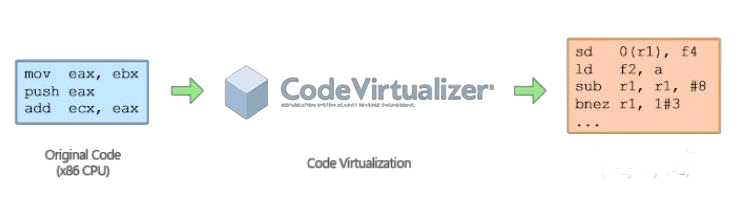
\includegraphics[width=.8\textwidth]
	{assets/pics/code_virtualization_process.png}
	\caption{Prosess Code Virtualization \cite{Ore06}}
	\label{F:virtualization_process}
\end{figure}
%-----------------------------------------------------------------------------%
\section{\f{Code Virtualization}}
%-----------------------------------------------------------------------------%

Code Virtualization atau juga disebut dengan VM-Based Code Obfuscation menerupakan suatu teknik obfuscation dimana kita menerjemahkan kode biner orignal menjadi bytecode baru berdasarkan Instruction Set Architecture (ISA) khusus (Gambar \ref{F:virtualization_process}). Bytecode ini dapat dijalankan secara run-time dengan mesin virtual (i.e. intrepreter) yang tertanam pada aplikasinya \cite{Ore06,Zho24}. Teknik Code virtualization tidak akan mengembalikan sumber kode aslinya dalam memori sedangkan teknik Code Encryption tetap mengembalikan kodenya aslinya dalam memori saat dilakukan dekripsinya \cite{Don20}.

Set instruksi virtual ini merupakan kunci dari obfuscationnya yang digunakan untuk mapping relasi antara intruksi lokal dan instruksi virtual \cite{Zho24} . Intruksi virtual ini membuat aliran kontrol dari original program untuk tidak dapat dibaca dan mempersulit reverse-engineer program. Code Virtualization dapat menghasilkan berbagai mesin virtual dengan set instruksi virtual masing-masing. Dengan ini, setiap copy dari program dapat memiliki instruksi virtual khusus agar mencegah penyerang untuk mengenali opcode mesin virtual menggunakan metode Frequency Analysis \cite{Ore06,Zho24}.

\begin{figure}
	\centering
	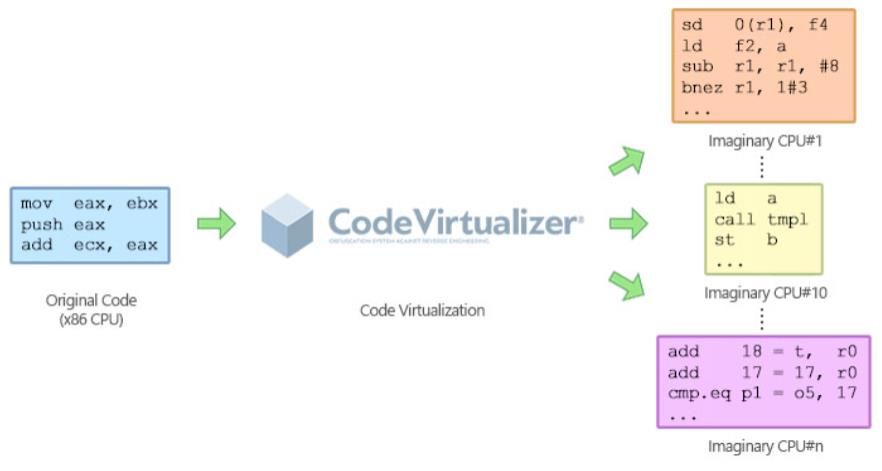
\includegraphics[width=1\textwidth]
	{assets/pics/multiple_virtualization.jpg}
	\caption{Transformasi ISA x86 menjadi berbagai messin virtual \cite{Ore06}}
\end{figure}

Arsitektur umum mesin virtual untuk Code Virtualization memiliki komponen-komponen yang mirip dengan design CPU \cite{Sal18, Hac24}.
\begin{enumerate}
	\item \bi{VM entry:} Perannya untuk simpan konteks eksekusi native (seperti register CPU atau flag) dan transisi ke konteks mesin virtual.
	\item \bi{Fetch:} Perannya adalah untuk mengambil, dari memori internal VM, opcode (virtual) yang akan ditiru, berdasarkan nilai Virtual Program Counter (vpc).
	\item \bi{Decode:} Perannya adalah untuk mendekode opcode yang diambil dan operan yang sesuai untuk menentukan instruksi ISA mana yang akan dieksekusi.
	\item \bi{Dispatch:} Setelah instruksi didekodekan, operator menentukan pengendali mana yang harus dijalankan dan mengatur konteksnya.
	\item \bi{Handlers:} Meniru instruksi virtual melalui rangkaian instruksi asli dan memperbarui konteks internal VM, biasanya vpc.
	\item \bi{VM exit:} Perannya untuk transisi dari konteks mesin virtual balik ke konteks eksekusi native.
\end{enumerate}

Proses eksekusi Code Virtualization pada program dapat dilihat pada Gambar \ref{F:execution_virtualization} dan contoh code virtualization pada intel assembly dapat dilihat pada Gambar \ref{F:transformation_virtualization}.

\begin{figure}
	\centering
	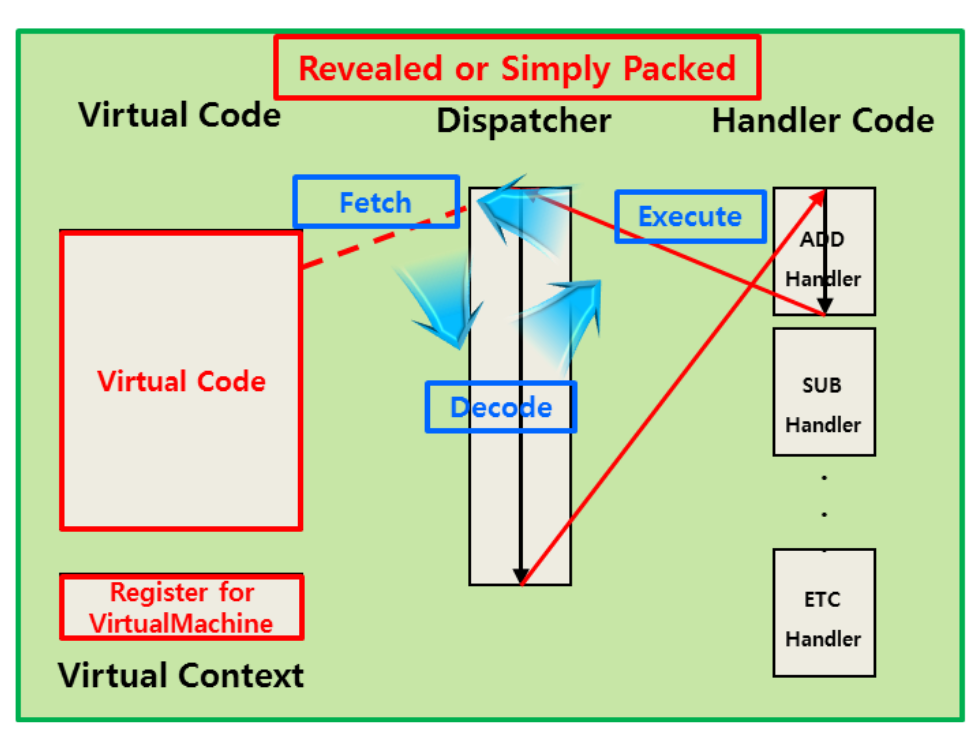
\includegraphics[width=0.7\textwidth]
	{assets/pics/virtualization_execution.png}
	\caption{Alur eksekusi Code Virtualization \cite{Don20}}
	\label{F:execution_virtualization}
\end{figure}

\begin{figure}
	\centering
	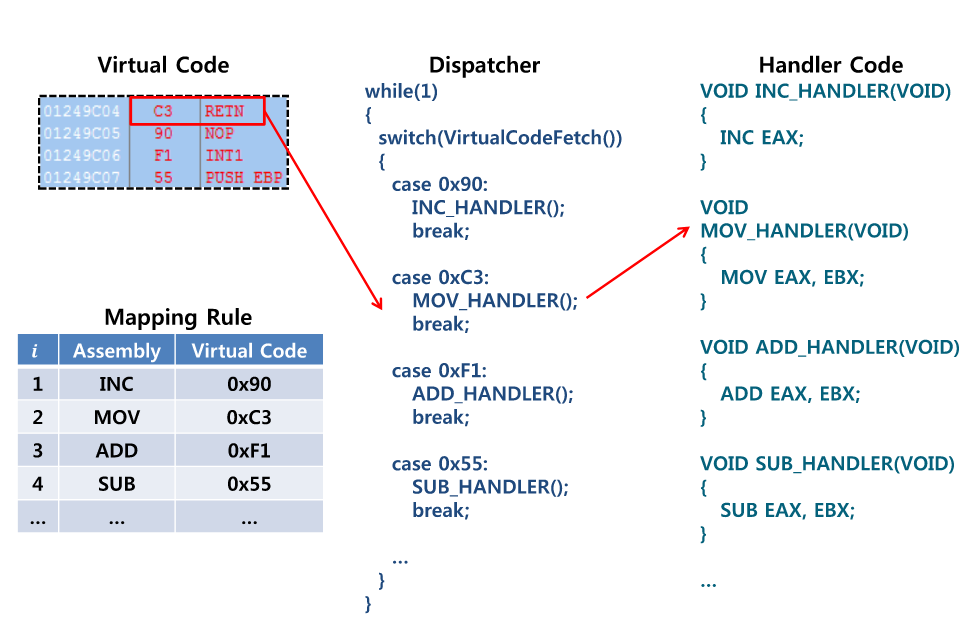
\includegraphics[width=0.7\textwidth]
	{assets/pics/code_to_virtualized.png}
	\caption{Transformasi kode asli menjadi kode virtual \cite{Don20}}
	\label{F:transformation_virtualization}
\end{figure}

\subsection{VxLang}
VxLang adalah sebuah proyek obfuscation kode atau biner yang bertujuan untuk mencegah attacker melakukan tindakan reverse engineering, seperti analisis statis atau dinamis, perusakan file, dan akses ilegal ke memori. VxLang ini merupakan sebuah perangkat komprehensif yang terdiri dari packer/protector, alat obfuscation kode, dan alat virtualisasi kode. Proyek ini saat ini menargetkan executable Microsoft Windows PE (.exe/.dll/*.sys dan UEFI) pada x86-64, dengan dukungan untuk Linux ELF dan ARM yang direncanakan di masa mendatang.
\subsubsection{Komponen-Komponen Utama VxLang}
VxLang terdiri dari beberapa komponen utama yang bekerja sama untuk melindungi kode:
\begin{itemize}
	\item \bi{Binary Protector:} Komponen ini memodifikasi, mengompresi, dan mengenkripsi executable asli menjadi format file yang digunakan secara internal oleh VxLang. Binary Protector juga menggabungkan kode inti VxLang, yang dapat diperkuat dan diperluas dengan modul tambahan. Struktur fleksibel ini memungkinkan pengguna untuk dengan bebas memperluas fungsionalitas dan mengontrol inti VxLang.
	\item \bi{Code Obfuscator:} Alat Obfuscation Kode ini mengubah kode native untuk menghalangi analisis, baik dengan memecah blok kode atau meratakan kode ke kedalaman yang sama. Metode obfuscation tambahan akan ditambahkan di masa mendatang. Obfuscation bertujuan untuk membuat kode lebih sulit dipahami tanpa mengubah fungsionalitasnya.
	\item \bi{Code Virtualizer:} Alat Virtualisasi Kode ini mengubah kode menjadi bahasa assembly internal. Bahasa ini kemudian dikonversi menjadi bytecode dan dieksekusi oleh compiler internal. Virtualisasi kode menambahkan lapisan abstraksi yang signifikan, sehingga mempersulit reverse engineering karena attacker harus memahami mesin virtual VxLang untuk dapat memahami kode yang dilindungi.
\end{itemize}

\subsubsection{Arsitektur dan Cara Kerja VxLang}

\begin{itemize}
	\item \bo{Proteksi Biner:} Binary Protector mengambil executable asli dan mengubahnya menjadi format internal VxLang. Proses ini dapat mencakup kompresi untuk mengurangi ukuran file, enkripsi untuk melindungi konten, dan modifikasi struktur file untuk mempersulit analisis statis. Dengan mengubah format file, VxLang mempersulit alat reverse engineering standar untuk memproses dan menganalisis executable.
	\item \bo{Obfuscation Kode:} Code Obfuscator mengubah kode native untuk membuatnya lebih sulit dipahami. Teknik-teknik yang digunakan dapat mencakup:
	      \begin{itemize}
		      \item \bo{Memecah blok kode:} Ini melibatkan pemisahan blok kode yang berurutan menjadi bagian-bagian yang lebih kecil dan menyisipkan lompatan di antara bagian-bagian tersebut. Hal ini mengganggu alur kontrol program dan mempersulit reverse engineer untuk mengikuti logika program.
		      \item \bo{Meratakan kode ke kedalaman yang sama (Code Flattening):} Ini melibatkan pengubahan struktur alur kontrol bersarang (misalnya, loop dan percabangan) menjadi urutan instruksi yang lebih datar. Hal ini menghilangkan hierarki dalam kode dan membuatnya lebih sulit untuk dipahami.
	      \end{itemize}
	      \begin{figure}[!htb]
		      \begin{minipage}{0.5\textwidth}
			      \centering
			      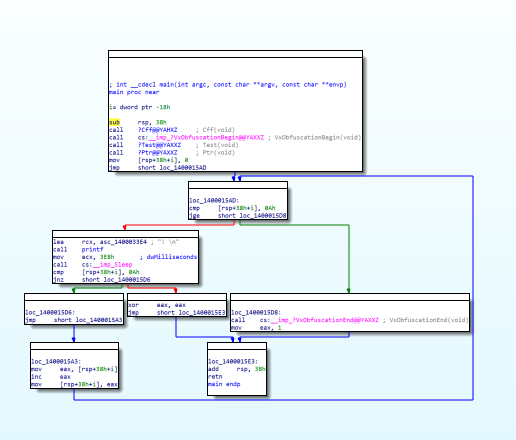
\includegraphics[width=0.8\linewidth]
			      {assets/pics/vxlang_before_flattening.PNG}
		      \end{minipage}\hfill
		      \begin{minipage}{0.5\textwidth}
			      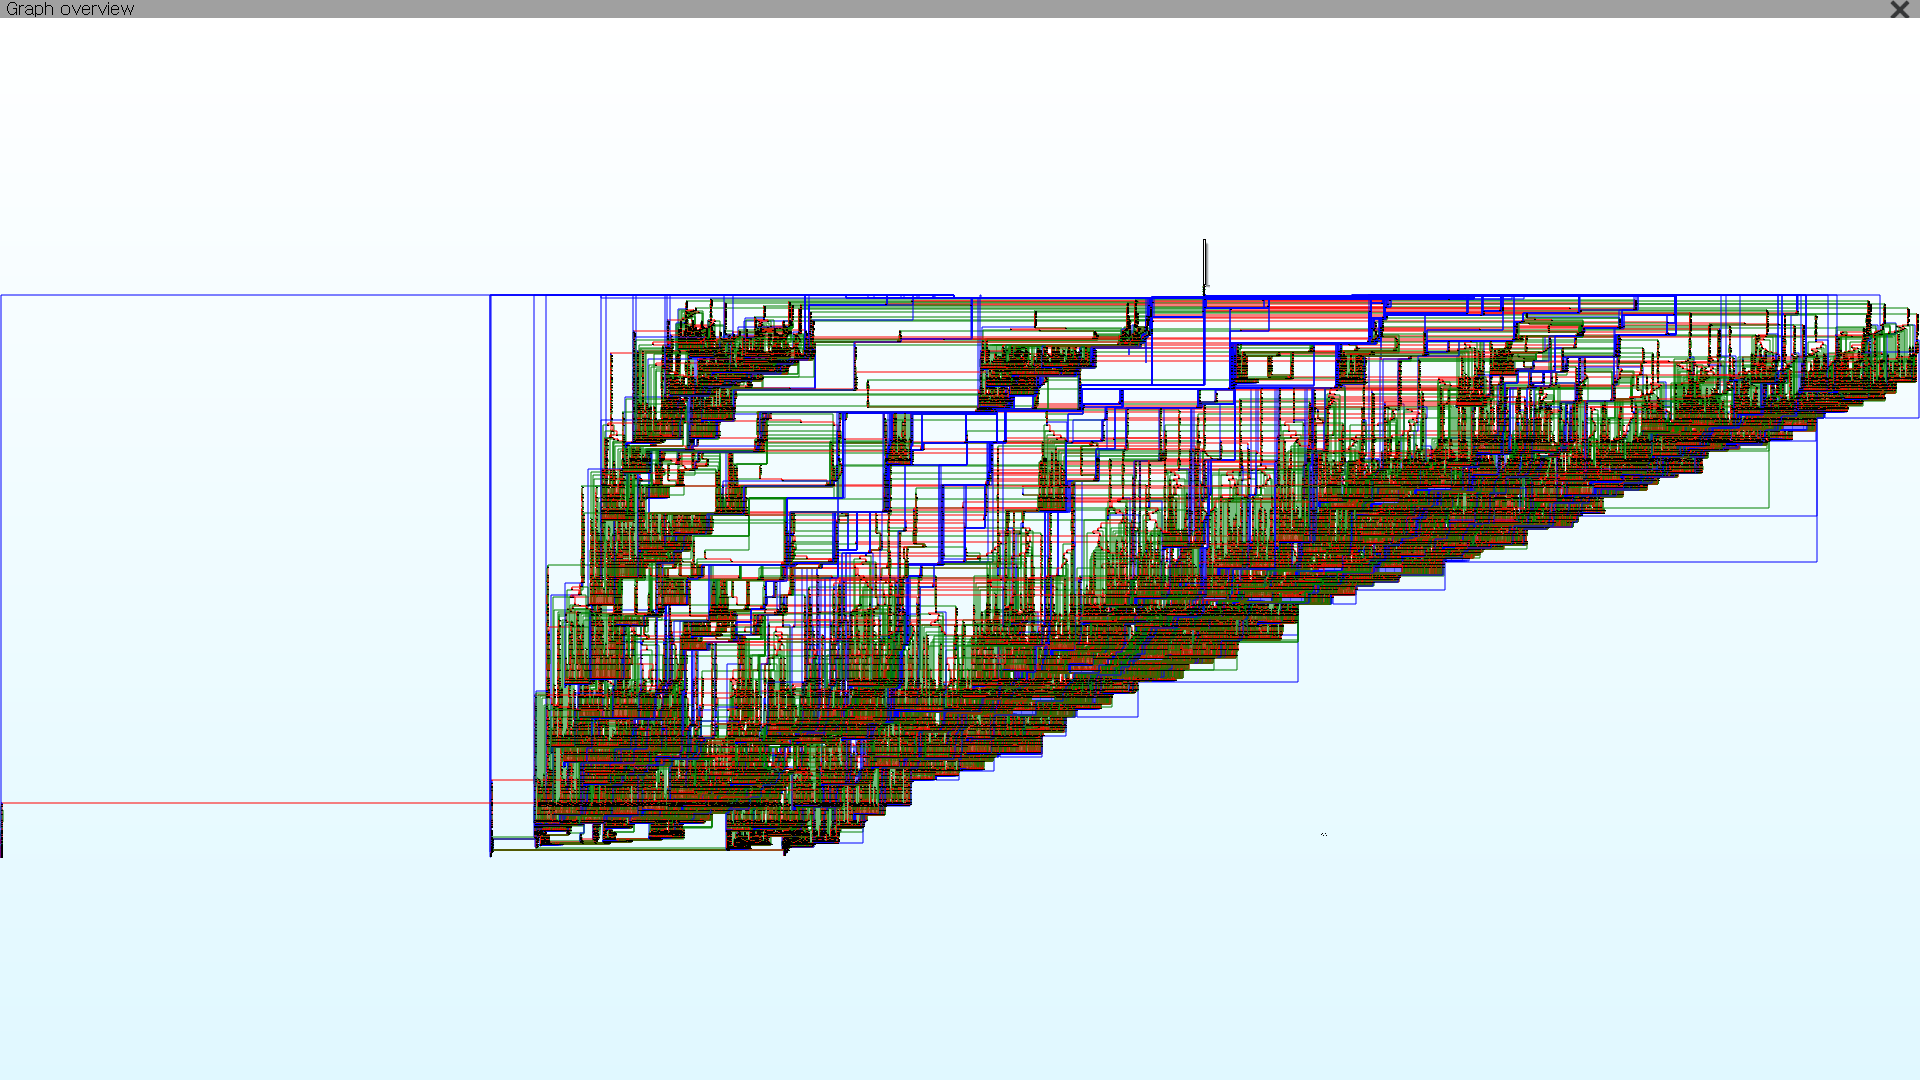
\includegraphics[width=1.0\linewidth]
			      {assets/pics/vxlang_after_flattening.png}
		      \end{minipage}
		      \caption{Sebelum dan Sesudah \textit{Obfuscation} \cite{VxLang}}
	      \end{figure}
	\item \bo{Virtualisasi kode:} Code Virtualizer mengubah kode native menjadi bytecode untuk mesin virtual VxLang. Bytecode ini kemudian dieksekusi oleh interpreter mesin virtual. Virtualisasi kode menambahkan lapisan abstraksi yang signifikan, karena attacker tidak lagi dapat menganalisis kode native secara langsung. Sebaliknya, mereka harus memahami arsitektur dan set instruksi mesin virtual VxLang, yang tidak terdokumentasi dan dapat dikustomisasi.
	      \begin{figure}
		      \centering
		      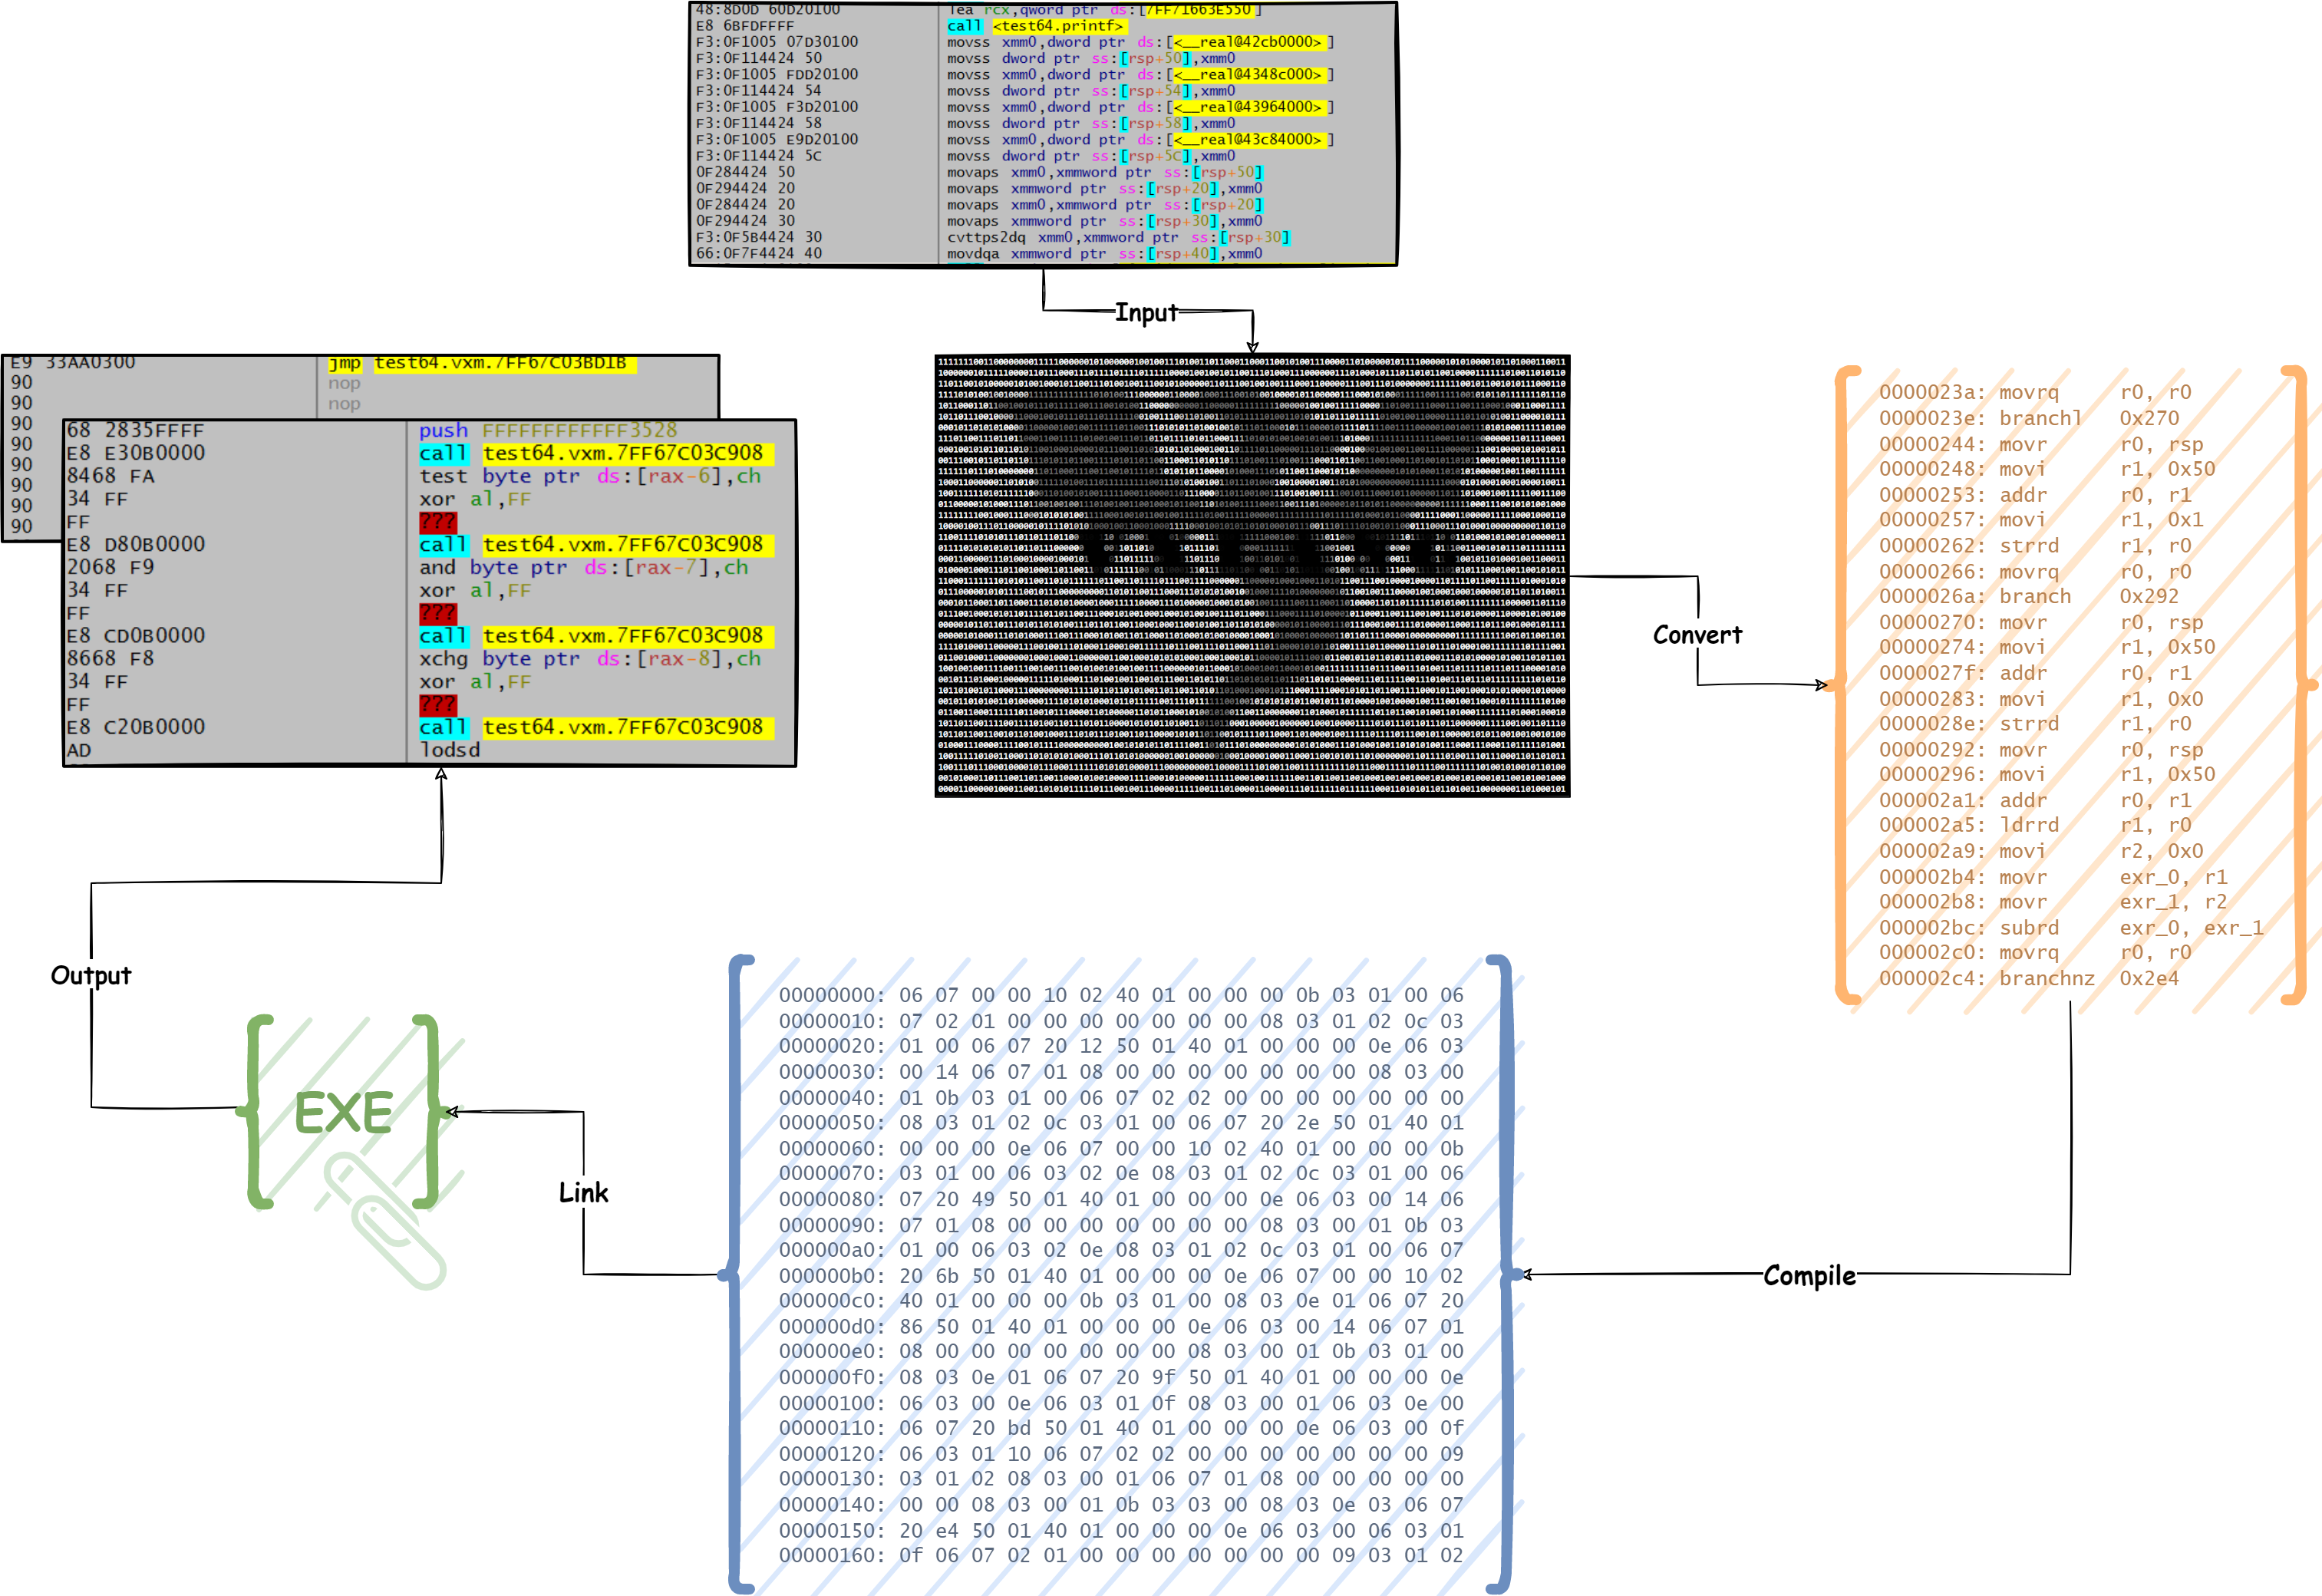
\includegraphics[width=0.55\textheight]
		      {assets/pics/vxlang_virtualizer.png}
		      \caption{VxLang \textit{Code Virtualizer} \cite{VxLang}}
	      \end{figure}
\end{itemize}

\subsubsection{VxLang SDK dan API untuk Obfuscation}
Untuk menggunakan VxLang, pengembang dapat menggunakan Software Development Kit (SDK) yang tersedia. SDK ini dapat diperoleh dengan mengunduh library yang telah dikompilasi atau dengan mendapatkan kode sumber dari GitHub dan membangunnya sendiri. Setelah mendapatkan SDK, langkah selanjutnya adalah mengatur header dan library links dalam kode proyek. \\

Di dalam header SDK, terdapat beberapa Application Programming Interfaces (API) yang berperan penting dalam melakukan obfuscation kode. API-API ini memungkinkan pengembang untuk menerapkan berbagai teknik obfuscation secara terarah pada kode sumber. Berikut adalah penjelasan mengenai API-API tersebut:

\begin{itemize}
	\item \bo{VL\_OBFUSCATION\_BEGIN/END:} API ini digunakan untuk menambahkan kode dummy (kode palsu) di antara kode asli. Penambahan kode dummy ini bertujuan untuk mengganggu proses disassembly dan decompilation. Disassembly adalah proses menerjemahkan kode mesin kembali ke dalam bentuk assembly, sedangkan decompilation adalah proses menerjemahkan kode mesin atau bytecode ke dalam bahasa pemrograman tingkat tinggi. Dengan adanya kode dummy, reverse engineer akan kesulitan untuk memahami alur eksekusi program yang sebenarnya karena kode dummy tersebut akan muncul dalam hasil disassembly dan decompilation, sehingga mengaburkan kode asli.
	      \begin{minted}
{cpp}     
          void obfuscation_test(int x) {

            VL_OBFUSCATION_BEGIN;

            printf("Obfuscation Test!")

            VL_OBFUSCATION_END;

          }
    \end{minted}
	\item \bo{VL\_CODE\_FLATTENING\_BEGIN/END:} API ini digunakan untuk mengacak urutan kode pada tingkat kedalaman yang sama. Proses ini juga melibatkan penambahan kode dummy dan membuat kode menjadi lebih sulit diinterpretasikan. Code flattening adalah teknik obfuscation yang mengubah struktur alur kontrol program menjadi lebih datar dan kompleks. Dengan mengacak urutan kode dan menambahkan kode dummy, reverse engineer akan kesulitan untuk merekonstruksi alur logika program yang sebenarnya.
	      \begin{minted}
{cpp}     
          void code_flattening_test(int x) {

            VL_CODE_FLATTENING_BEGIN;

            printf("Code Flattening Test!")

            VL_CODE_FLATTENING_END;

          }
    \end{minted}
	\item \bo{VL\_VIRTUALIZATION\_BEGIN/END:} API ini digunakan untuk mengubah kode native yang ditentukan menjadi bytecode yang hanya dapat diinterpretasikan oleh Central Processing Unit (CPU) internal VxLang. Ini adalah inti dari teknik virtualisasi kode yang ditawarkan oleh VxLang. Kode native yang telah diubah menjadi bytecode tidak lagi dapat dieksekusi secara langsung oleh prosesor fisik, melainkan harus melalui interpreter mesin virtual VxLang. Ini secara signifikan meningkatkan kesulitan reverse engineering karena attacker harus memahami arsitektur dan set instruksi mesin virtual VxLang untuk dapat memahami kode yang dilindungi.
	      \begin{minted}
{cpp}     
          void virtualization_test(int x) {

            VL_VIRTUALIZATION_BEGIN;

            printf("Virtualization Test!")

            VL_VIRTUALIZATION_END;

          }
    \end{minted}

\end{itemize}

API-API ini dapat diterapkan pada kode sumber dengan cara menandai bagian-bagian kode yang ingin diobfuskasi atau divirtualisasi dengan menggunakan API BEGIN dan END yang sesuai.

\subsubsection{Konfigurasi Obfuscation VxLang}
VxLang menawarkan dua mode penggunaan: Command Line Mode dan Project Mode. Command Line Mode relatif sederhana, sedangkan Project Mode memungkinkan pengembang untuk mengatur proyek mereka melalui file JSON. Dalam penjelasan ini, kita akan fokus pada Project Mode.

Project Mode menggunakan file JSON untuk mengkonfigurasi berbagai aspek dari proses obfuscation dan virtualisasi.
\begin{figure}
	\centering
	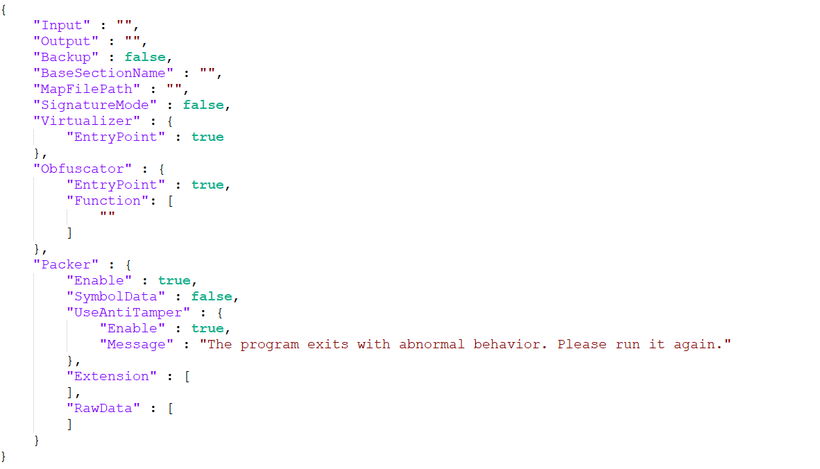
\includegraphics[width=0.55\textheight]
	{assets/pics/vxlang_json.png}
	\caption{VxLang konfigurasi JSON \cite{VxLang}}
\end{figure}
Berikut adalah penjelasan mengenai pengaturan-pengaturan yang terdapat dalam file JSON konfigurasi:
\begin{itemize}
	\item \bo{Input :} Menentukan path (jalur) ke file kode sumber yang akan diproses.
	\item \bo{Output :} Menentukan path ke file keluaran (output) yang telah diobfuskasi.
	\item \bo{Backup :} Flag (bendera) yang menentukan apakah file kode sumber asli perlu di-backup (dicadangkan).
	\item \bo{BaseSectionName :} Nama bagian (section) yang menjadi dasar. Jika diatur ke ".base", nama bagian VxLang akan ditulis sebagai ".base0"/".base1". Section adalah bagian-bagian dalam file executable yang menyimpan kode, data, dan informasi lainnya.
	\item \bo{MapFilePath :} Path ke file map. File map berisi informasi mengenai alamat dan simbol dalam program, yang dapat digunakan untuk debugging atau analisis.
	\item \bo{SignatureMode :} Kemampuan untuk melakukan obfuscation dengan menambahkan tanda tangan (signature) dalam lingkungan di mana SDK tidak dapat ditemukan (misalnya, bahasa native yang berbeda). Signature dapat digunakan untuk memverifikasi integritas kode atau untuk keperluan lisensi.
	\item \bo{Virtualizer :} Pengaturan untuk fitur virtualisasi.
	      \begin{itemize}
		      \item \bo{EntryPoint :} Memvirtualisasi entry point program. Entry point adalah alamat memori tempat eksekusi program dimulai. Memvirtualisasi entry point dapat mempersulit attacker untuk memahami bagaimana program dimulai dan bagaimana alur kontrol program diinisialisasi.
	      \end{itemize}
	\item \bo{Obfuscator :} Pengaturan untuk code flattening atau obfuscation umum.
	      \begin{itemize}
		      \item \bo{EntryPoint :} Meng-obfuscasi entry point program.
		      \item \bo{Function :} Meng-obfuscasi fungsi-fungsi tertentu yang dipilih dalam file map.
	      \end{itemize}
	\item \bo{Packer :} Pengaturan untuk kompresi dan obfuscation biner. Packer adalah program yang mengompresi dan/atau meng-obfuscasi file executable untuk mempersulit reverse engineering.
	      \begin{itemize}
		      \item \bo{Enable :} Flag yang menentukan apakah biner perlu dikompresi.
	      \end{itemize}
	\item \bo{SymbolData :} Flag yang menentukan apakah simbol-simbol debugging perlu dicatat (logged). Simbol-simbol debugging berisi informasi yang berguna untuk debugging, tetapi juga dapat membantu reverse engineer dalam memahami kode.
	\item \bo{UseAntiTemper :} Pengaturan untuk fitur anti-tamper. Anti-tamper adalah teknik untuk mencegah atau mendeteksi modifikasi yang tidak sah pada kode.
	      \begin{itemize}
		      \item \bo{Enable :} Nilai yang menentukan apakah fitur anti-tamper diaktifkan.
		      \item \bo{Message :} Pesan deteksi yang akan ditampilkan ketika deteksi oleh fitur deteksi tertentu.
	      \end{itemize}
	\item \bo{extension :} Daftar modul ekstensi VxLang. Modul ekstensi dapat digunakan untuk menambahkan fungsionalitas tambahan ke VxLang.
	\item \bo{RawData :} Daftar data yang menyertai modul ekstensi. Daftar ini tersedia dalam modul ekstensi.
\end{itemize}

\section{\textit{Graphical User Interface Frameworks}}
Dalam pengembangan aplikasi autentikasi sebagai bagian dari demonstrasi pada penelitian ini, digunakan dua framework antarmuka pengguna grafis (GUI) yang berbeda, yaitu Qt Framework dan Dear ImGUI.

\subsection{\textit{Qt Framework}}
Qt Framework adalah sebuah framework pengembangan aplikasi lintas platform yang sangat populer dan komprehensif. Berdasarkan dokumentasi \cite{Qt}, Qt menyediakan berbagai macam tool dan library yang diperlukan untuk mengembangkan aplikasi dengan antarmuka pengguna yang kaya dan interaktif, serta fungsionalitas non-GUI seperti akses database, jaringan, dan lainnya.

\noindent{\bo{Karakteristik \textit{Qt Framework}:}}
\begin{itemize}
	\item \bi{Cross Platform :} Salah satu keunggulan utama Qt adalah kemampuannya untuk berjalan di berbagai sistem operasi seperti Windows, Linux, macOS, Android, iOS, dan bahkan sistem embedded. Ini memungkinkan pengembang untuk menulis kode sekali dan menjalankannya di berbagai platform tanpa perlu modifikasi signifikan.
	\item \bo{Fitur yang Kaya :} Qt menyediakan berbagai macam widget dan layout untuk membangun antarmuka pengguna yang kompleks dan menarik. Selain itu, Qt juga menawarkan dukungan yang kuat untuk grafik 2D dan 3D, animasi, multimedia, dan integrasi dengan teknologi web.
	\item \bo{Bahasa Pemrograman Utama :} Qt umumnya digunakan dengan bahasa pemrograman C++, namun juga memiliki binding untuk bahasa lain seperti Python (melalui PyQt atau PySide).
\end{itemize}

Dalam konteks ini, Qt Framework digunakan untuk membangun antarmuka pengguna yang lebih tradisional dan mungkin lebih kompleks untuk aplikasi autentikasi. Ini memungkinkan visualisasi alur kerja autentikasi, input pengguna (seperti username dan password), dan tampilan hasil autentikasi dengan cara yang terstruktur dan mudah dipahami.

\begin{figure}
	\centering
	
\includegraphics[width=0.15\textheight]
	{assets/pics/Qt_logo.png}
	\caption{Qt Logo \cite{Qt}}
\end{figure}

\subsection{\textit{Dear ImGUI}}
Dear ImGUI adalah sebuah library antarmuka pengguna grafis (GUI) immediate mode yang ringan dan tidak memerlukan banyak boilerplate untuk digunakan. Berdasarkan repositori GitHub-nya \cite{ImGui}, Dear ImGUI dirancang untuk fokus pada kesederhanaan dan kemudahan integrasi ke dalam aplikasi yang sudah ada, terutama untuk keperluan debugging, tooling, atau prototipe cepat.

\noindent{\bo{Karakteristik \textit{Dear ImGUI}:}}
\begin{itemize}
	\item \bi{Immediate Mode GUI :} Berbeda dengan retained mode GUI seperti Qt, di mana widget dibuat dan dikelola secara eksplisit, Dear ImGUI bekerja dengan cara menggambar ulang seluruh antarmuka pada setiap frame. Ini membuat pengembangan UI menjadi lebih intuitif dan stateful secara implisit.
	\item \bo{Ringan dan Cepat :} Dear ImGUI memiliki ukuran library yang kecil dan performa yang baik, sehingga cocok untuk aplikasi yang membutuhkan sumber daya minimal atau yang sudah memiliki rendering engine sendiri.
	\item \bo{Fokus pada Fungsionalitas Inti :} Dear ImGUI menyediakan berbagai widget dasar seperti tombol, slider, teks input, dan window, yang cukup untuk membangun antarmuka pengguna yang fungsional untuk keperluan demonstrasi atau tooling.
\end{itemize}

Dear ImGUI digunakan untuk menampilkan informasi atau kontrol yang lebih teknis atau diagnostik terkait dengan proses autentikasi yang dilindungi oleh VxLang. Sifatnya yang ringan dan mudah diintegrasikan mungkin menjadikannya pilihan yang baik untuk menampilkan proses autentikasi.

\section{OpenSSL}
OpenSSL adalah sebuah toolkit yang kuat, berkualitas komersial, dan kaya fitur untuk protokol Transport Layer Security (TLS) dan Secure Sockets Layer (SSL). OpenSSL merupakan fondasi kriptografi open-source yang banyak digunakan dalam berbagai aplikasi dan sistem untuk mengamankan komunikasi melalui jaringan \cite{OpenSSL}.

\noindent{\bo{Karakteristik OpenSSL:}}
\begin{itemize}
	\item \bo{Toolkit Kriptograf :} OpenSSL menyediakan implementasi dari berbagai algoritma kriptografi, termasuk algoritma simetris (seperti AES), algoritma asimetris (seperti RSA dan ECC), fungsi hash kriptografi (seperti SHA-256), dan banyak lagi. Ini menjadikannya pilihan yang fleksibel untuk berbagai kebutuhan keamanan.
	\item \bo{Implementasi Standar Keamanan  :} OpenSSL mengimplementasikan protokol keamanan standar seperti TLS dan SSL, yang digunakan untuk mengenkripsi komunikasi antara klien dan server di internet, seperti pada protokol HTTPS.
\end{itemize}

\begin{figure}
	\centering
	
\includegraphics[width=0.25\textheight]
	{assets/pics/OpenSSL_logo.png}
	\caption{OpenSSL Logo \cite{OpenSSL}}
\end{figure}

OpenSSL dalam penelitian digunakan untuk menjalankan algoritma enkripsi AES (Advanced Encryption Standard) dengan mode CBC (Cipher Block Chaining) dan panjang kunci 256-bit digunakan dari library OpenSSL. AES adalah algoritma enkripsi simetris yang sangat aman dan banyak digunakan. Mode CBC merupakan salah satu mode operasi blok cipher yang umum digunakan dan memerlukan Initialization Vector (IV) acak untuk setiap proses enkripsi guna meningkatkan keamanan. Panjang kunci 256-bit memberikan tingkat keamanan yang sangat tinggi terhadap serangan brute-force.

Penggunaan enkripsi AES-CBC-256 dari OpenSSL dalam percobaan ini bertujuan untuk mengukur performance overhead (beban kinerja) yang mungkin ditimbulkan oleh penerapan VxLang. Dengan membandingkan waktu eksekusi operasi enkripsi yang sama sebelum dan sesudah kode dilindungi oleh VxLang, dapat dianalisis dampak virtualisasi kode terhadap kinerja aplikasi. Pemilihan algoritma AES-CBC-256 sebagai tolok ukur kemungkinan didasarkan pada popularitasnya, tingkat keamanannya, dan ketersediaannya dalam library OpenSSL yang banyak digunakan.
